\documentclass[a4paper,11pt]{article}

% 日本語対応
\usepackage{xeCJK}
\setCJKmainfont{Noto Sans CJK JP}

% 数学関連パッケージ
\usepackage{amsmath}
\usepackage{amssymb}
\usepackage{amsthm}
\usepackage{amsfonts}
\usepackage{mathtools}

% 図形描画用パッケージ
\usepackage{tikz}
\usepackage{pgfplots}
\pgfplotsset{compat=1.18}

% その他パッケージ
\usepackage{graphicx}
\usepackage{enumitem}
\usepackage{float}
\usepackage{hyperref}
\usepackage{fancyhdr}
\usepackage{geometry}

% ページ設定
\geometry{
  a4paper,
  top=25mm,
  bottom=25mm,
  left=25mm,
  right=25mm
}

% ヘッダーとフッターの設定
\pagestyle{fancy}
\fancyhf{}
\fancyhead[L]{数学問題}
\fancyhead[R]{\today}
\fancyfoot[C]{\thepage}
\renewcommand{\headrulewidth}{0.4pt}
\renewcommand{\footrulewidth}{0.4pt}

% タイトル情報
\title{数学問題}
\author{数学問題生成AIシステム}
\date{\today}

% ドキュメント開始
\begin{document}

\maketitle

% 問題セクション
\section*{問題}

% 問題文を挿入(変数で置換)
次の二次関数 $f(x) = x^2 - 4x + 3$ のグラフについて、頂点の座標を求めなさい。

% 解答セクション(オプショナル - 表示したくない場合はコメントアウト)
\section*{解答}

% 解答を挿入(変数で置換)
頂点の座標は $(2, -1)$ である。

% 解説セクション(オプショナル - 表示したくない場合はコメントアウト)
\section*{解説}

% 解説を挿入(変数で置換)
二次関数 $f(x) = x^2 - 4x + 3$ は $f(x) = (x - 2)^2 - 1$ と変形できる。
したがって、頂点の座標は $(2, -1)$ である。

% 図形が必要な場合はここに挿入
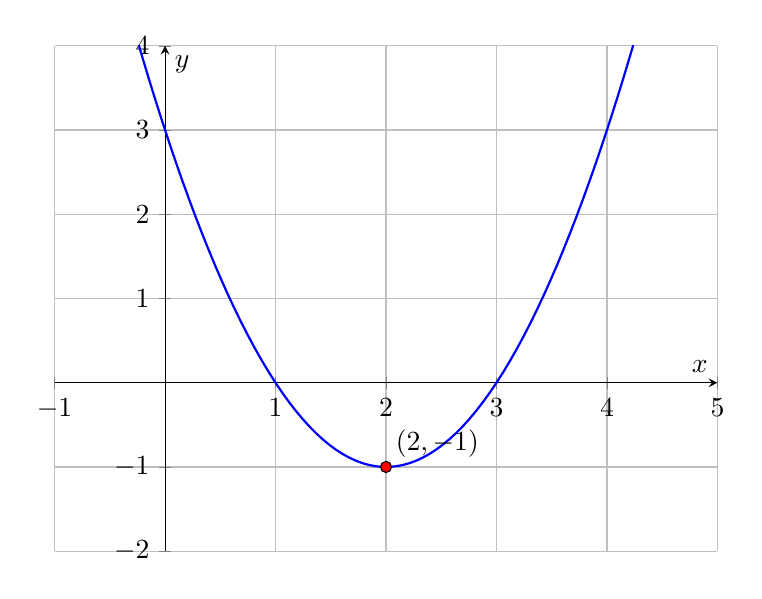
\begin{tikzpicture}
        \begin{axis}[
          axis lines=middle,
          xlabel=$x$,
          ylabel=$y$,
          xmin=-1, xmax=5,
          ymin=-2, ymax=4,
          grid=both,
          width=10cm,
          height=8cm
        ]
          \addplot[domain=-1:5, samples=100, blue, thick] {x^2 - 4*x + 3};
          \addplot[mark=*, fill=red] coordinates {(2,-1)} node[above right] {$(2,-1)$};
        \end{axis}
      \end{tikzpicture}

\end{document} 